\chapter{Dataset proposto}
\label{new_dataset}
\section{Motivazione e composizione}
Per creare questo nuovo dataset sono state raccolte 146 nuove immagini, di cui 85 scattate da un fotografo professionista e 61 scattate da utenti non professionisti. É stato poi estrapolato da esse un sottoinsieme di 100 immagini, rispettivamente 50 professionali e 50 amatoriali, per poterle usare per valutare la capacità di generalizzazione della rete neurale che verrà usata successivamente.

Il motivo per cui si è scelto di proporre un nuovo dataset è stato quello di conoscere le prestazioni ottenute con la rete neurale, precedentemente utilizzata con il test set estratto dal GPD, e un nuovo set di immagini che la rete non avesse mai visto. Una particolarità evidente di questo dataset è il fatto che sia composto sia da fotografie professionali che da fotografie amatoriali, questo perché si è scelto di investigare il tema dell'estetica cercando di capire se la modalità di acquisizione e la tecnica fotografica possano influenzarne la percezione.

Le fotografie professionali sono state scattate nel corso degli anni da un fotografo professionista con macchine fotografiche Canon e principalmente con una lente a lunghezza focale fissa (50mm, 85mm o 100mm), che in questo caso permette di mettere a fuoco il soggetto e ottenere un effetto sfocato nel background, inoltre sono state precedentemente selezionate e contengono enhancement in quanto sono state scattate per menù e social network di ristoranti ed eventi perciò sono state necessarie queste operazioni prima di consegnarle agli utilizzatori finali.

Le fotografie amatoriali provengono da viaggi ed esperienze personali, sono state scattate principalmente da me in prima persona con iPhone 8 e iPhone 12 Pro oppure, in minima parte, da amici e non contengono enhancement di alcun tipo.

\section{Assegnamento delle groundtruth}
Inizialmente si pensava che le fotografie professionali fossero esteticamente belle, mentre quelle scattate dagli utenti non lo fossero, ma per confermare questa ipotesi è stato richiesto l'intervento di 41 utenti che valutassero le immagini in modo tale da ottenere le vere e proprie groundtruth, le quali potevano coincidere o meno con quelle ipotizzate inizialmente.
%Al fine di assegnare le label di groundtruth alle immagini del nuovo dataset,

\begin{comment}
\begin{figure}[H]
\centering
% scale= 0.72
% scale= 0.69
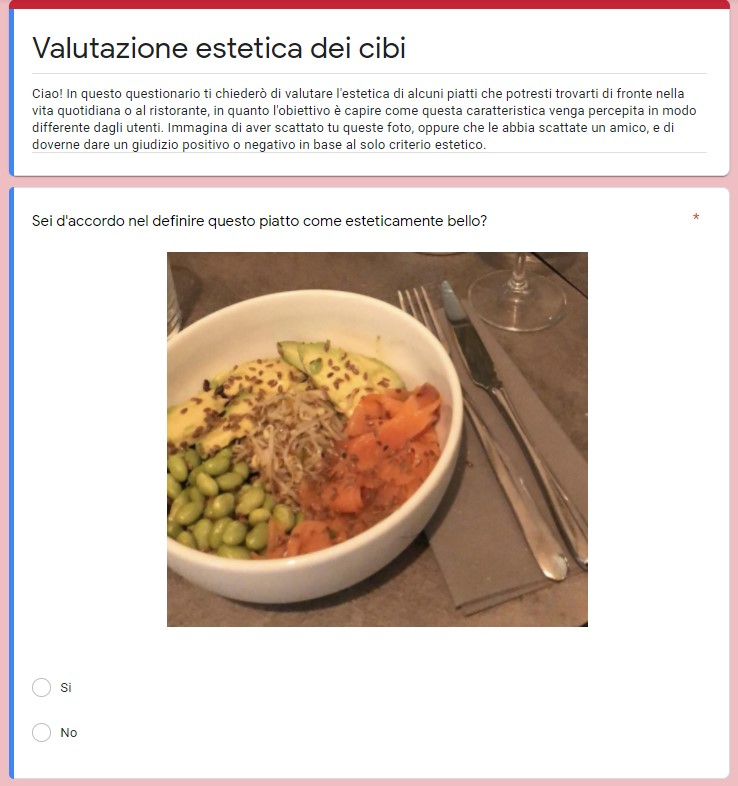
\includegraphics[scale= 0.69]{images/domanda questionario1.jpg}
\caption{Esempio di una delle domande del questionario che è servito per far valutare a 41 utenti le immagini del dataset proposto e ottenere le label di groundtruth}
\label{questionario1}
\end{figure}
\end{comment}

% inserimento Mock
\begin{figure}[H]
\centering
% scale=0.27
\includegraphics[scale=0.25]{images/mockup/Mockup_Q1.png}
\quad
\includegraphics[scale=0.25]{images/mockup/Mockup_D2Q1.png}
\quad
\caption{Esempio di una delle domande del questionario che è servito per far valutare a 41 utenti le immagini del dataset proposto e ottenere le label di groundtruth}
\label{questionario1}
\end{figure}

Prendendo ispirazione dallo stato dell'arte e da altri lavori sull'estetica \cite{sheng2021learning},  è stato creato un questionario all'interno del quale gli utenti hanno votato se, in base alla loro opinione e alla loro percezione dell'estetica, i piatti potevano essere considerati esteticamente belli o meno e, quindi, appartenere alla classe positiva o negativa. In base a questi voti sono state assegnate le label, in particolare per ogni immagine I$_i$ la corrispondente label binaria \^y$_{i}$ è data dalla maggioranza dei voti relativi a quella specifica immagine. Un esempio di una domanda del questionario è visibile in Figura \ref{questionario1}.

Di seguito, in Figura \ref{negativeNew}, sono riportate tutte le 27 immagini del dataset che  sono risultate avere una groundtruth negativa, mentre in Figura \ref{positiveNew} sono riportate tutte le 73 immagini che hanno groundtruth positiva. Si noti che nonostante si sia partiti da 50 immagini professionali e 50 amatoriali alla fine la numerosità di immagini con groundtruth negativa è minore di quella con groundtruth positiva, in quanto gli utenti hanno valutato positivamente anche alcune fotografie non professionali, ipoteticamente non concentrandosi sulla fotografia in sé bensì sul cibo stesso e pensando se quello specifico cibo fosse di loro gradimento. In minima parte ci sono stati anche casi in cui fotografie professionali sono state valutate negativamente.

% INSERIMENTO DI TUTTE LE IMMAGINI DEL DATASET
% negative
\begin{figure}[H]
\centering
\includegraphics[height=35mm]{images/new dataset/negative/negative (1).jpg}
\quad
\includegraphics[height=35mm]{images/new dataset/negative/negative (2).jpg}
\quad
\vspace{5mm}
\includegraphics[height=35mm]{images/new dataset/negative/negative (3).jpg}
\quad
\includegraphics[height=35mm]{images/new dataset/negative/negative (4).jpg}
\quad
\vspace{5mm}
\includegraphics[height=35mm]{images/new dataset/negative/negative (5).jpg}
\quad
\includegraphics[height=35mm]{images/new dataset/negative/negative (6).jpg}
\quad
\includegraphics[height=35mm]{images/new dataset/negative/negative (7).jpg}
\quad
\vspace{5mm}
\includegraphics[height=35mm]{images/new dataset/negative/negative (8).jpg}
\quad
\includegraphics[height=35mm]{images/new dataset/negative/negative (9).jpg}
\quad
\end{figure}

% vanno splittate per gestire la fine della pagina 
\begin{figure}[H]
\centering
\includegraphics[height=35mm]{images/new dataset/negative/negative (10).jpg}
\quad
\includegraphics[height=35mm]{images/new dataset/negative/negative (11).jpg}
\quad
\includegraphics[height=35mm]{images/new dataset/negative/negative (12).jpg}
\quad
\includegraphics[height=35mm]{images/new dataset/negative/negative (13).jpg}
\quad
\vspace{5mm}

\includegraphics[height=35mm]{images/new dataset/negative/negative (14).jpg}
\quad
\includegraphics[height=35mm]{images/new dataset/negative/negative (15).jpg}
\quad
\includegraphics[height=35mm]{images/new dataset/negative/negative (16).jpg}
\quad
\vspace{5mm}
\includegraphics[height=35mm]{images/new dataset/negative/negative (17).jpg}
\quad
%%
\includegraphics[height=35mm]{images/new dataset/negative/negative (18).jpg}
\quad
\includegraphics[height=35mm]{images/new dataset/negative/negative (19).jpg}
\quad
\includegraphics[height=35mm]{images/new dataset/negative/negative (20).jpg}
\quad 
\vspace{5mm}
\includegraphics[height=35mm]{images/new dataset/negative/negative (21).jpg}
\quad
\includegraphics[height=35mm]{images/new dataset/negative/negative (22).jpg}
\quad
\vspace{5mm}
\includegraphics[height=35mm]{images/new dataset/negative/negative (23).jpg}
\quad
\includegraphics[height=35mm]{images/new dataset/negative/negative (24).jpg}
\quad
%\vspace{5mm}
\includegraphics[height=35mm]{images/new dataset/negative/negative (25).jpg}
\quad
\includegraphics[height=35mm]{images/new dataset/negative/negative (26).jpg}
\quad
\includegraphics[height=35mm]{images/new dataset/negative/negative (27).jpg}
\caption{Immagini del dataset a cui è stata assegnata una groundtruth negativa tramite i voti degli utenti}
\label{negativeNew}
\end{figure}

% positive
\begin{figure}[H]
\centering
\includegraphics[height=35mm]{images/new dataset/positive/positive (1).jpg}
\quad
\includegraphics[height=35mm]{images/new dataset/positive/positive (2).jpg}\quad
\includegraphics[height=35mm]{images/new dataset/positive/positive (3).jpg}\quad
\vspace{5mm}
\includegraphics[height=35mm]{images/new dataset/positive/positive (4).jpg}\quad
\includegraphics[height=35mm]{images/new dataset/positive/positive (5).jpg}\quad
\includegraphics[height=35mm]{images/new dataset/positive/positive (6).jpg}\quad
\vspace{5mm}
\includegraphics[height=35mm]{images/new dataset/positive/positive (7).jpg}\quad
\includegraphics[height=35mm]{images/new dataset/positive/positive (8).jpg}\quad
\vspace{5mm}
\includegraphics[height=35mm]{images/new dataset/positive/positive (9).jpg}\quad
\includegraphics[height=35mm]{images/new dataset/positive/positive (10).jpg}\quad
\vspace{5mm}
\includegraphics[height=35mm]{images/new dataset/positive/positive (11).jpg}\quad
\includegraphics[height=35mm]{images/new dataset/positive/positive (12).jpg}\quad
\includegraphics[height=35mm]{images/new dataset/positive/positive (13).jpg}\quad
\vspace{5mm}
\includegraphics[height=35mm]{images/new dataset/positive/positive (14).jpg}\quad
\includegraphics[height=35mm]{images/new dataset/positive/positive (15).jpg}\quad
\end{figure}

\begin{figure}[H]
\centering
\includegraphics[height=35mm]{images/new dataset/positive/positive (16).jpg}\quad
\includegraphics[height=35mm]{images/new dataset/positive/positive (17).jpg}\quad
\vspace{5mm}
\includegraphics[height=35mm]{images/new dataset/positive/positive (18).jpg}\quad
\includegraphics[height=35mm]{images/new dataset/positive/positive (19).jpg}\quad
\includegraphics[height=35mm]{images/new dataset/positive/positive (20).jpg}\quad
\vspace{5mm}
\includegraphics[height=35mm]{images/new dataset/positive/positive (21).jpg}
\quad
\includegraphics[height=35mm]{images/new dataset/positive/positive (22).jpg}\quad
\includegraphics[height=35mm]{images/new dataset/positive/positive (23).jpg}\quad
\vspace{5mm}
\includegraphics[height=35mm]{images/new dataset/positive/positive (24).jpg}\quad
\includegraphics[height=35mm]{images/new dataset/positive/positive (25).jpg}\quad
\includegraphics[height=35mm]{images/new dataset/positive/positive (26).jpg}\quad
\vspace{5mm}
\includegraphics[height=35mm]{images/new dataset/positive/positive (27).jpg}\quad
\includegraphics[height=35mm]{images/new dataset/positive/positive (28).jpg}\quad
\includegraphics[height=35mm]{images/new dataset/positive/positive (29).jpg}\quad
\includegraphics[height=35mm]{images/new dataset/positive/positive (30).jpg}\quad
\includegraphics[height=35mm]{images/new dataset/positive/positive (31).jpg}\quad
\includegraphics[height=35mm]{images/new dataset/positive/positive (32).jpg}\quad
\includegraphics[height=35mm]{images/new dataset/positive/positive (33).jpg}\quad
\end{figure}

\begin{figure}[H]
\centering
\includegraphics[height=35mm]{images/new dataset/positive/positive (34).jpg}\quad
\includegraphics[height=35mm]{images/new dataset/positive/positive (35).jpg}
\quad
\includegraphics[height=35mm]{images/new dataset/positive/positive (36).jpg}\quad
\vspace{5mm}
\includegraphics[height=35mm]{images/new dataset/positive/positive (37).jpg}\quad
\includegraphics[height=35mm]{images/new dataset/positive/positive (38).jpg}\quad
\includegraphics[height=35mm]{images/new dataset/positive/positive (39).jpg}\quad
\vspace{5mm}
\includegraphics[height=35mm]{images/new dataset/positive/positive (40).jpg}\quad
\includegraphics[height=35mm]{images/new dataset/positive/positive (41).jpg}\quad
\includegraphics[height=35mm]{images/new dataset/positive/positive (42).jpg}\quad
\vspace{5mm}
\includegraphics[height=35mm]{images/new dataset/positive/positive (43).jpg}\quad
\includegraphics[height=35mm]{images/new dataset/positive/positive (44).jpg}\quad
\vspace{5mm}
\includegraphics[height=35mm]{images/new dataset/positive/positive (45).jpg}\quad
\includegraphics[height=35mm]{images/new dataset/positive/positive (46).jpg}\quad
\vspace{5mm}
\includegraphics[height=35mm]{images/new dataset/positive/positive (47).jpg}\quad
\end{figure}

\begin{figure}[H]
\centering
\includegraphics[height=35mm]{images/new dataset/positive/positive (48).jpg}\quad
\includegraphics[height=35mm]{images/new dataset/positive/positive (49).jpg}\quad
\vspace{5mm}
\includegraphics[height=35mm]{images/new dataset/positive/positive (50).jpg}\quad
\includegraphics[height=35mm]{images/new dataset/positive/positive (51).jpg}\quad
\includegraphics[height=35mm]{images/new dataset/positive/positive (52).jpg}\quad
\vspace{5mm}
\includegraphics[height=35mm]{images/new dataset/positive/positive (53).jpg}
\quad
\vspace{5mm}
\includegraphics[height=35mm]{images/new dataset/positive/positive (54).jpg}\quad
\includegraphics[height=35mm]{images/new dataset/positive/positive (55).jpg}\quad
\includegraphics[height=35mm]{images/new dataset/positive/positive (56).jpg}\quad
\vspace{5mm}
\includegraphics[height=35mm]{images/new dataset/positive/positive (57).jpg}\quad
\includegraphics[height=35mm]{images/new dataset/positive/positive (58).jpg}\quad
\includegraphics[height=35mm]{images/new dataset/positive/positive (59).jpg}\quad
\includegraphics[height=35mm]{images/new dataset/positive/positive (60).jpg}\quad
\end{figure}

\begin{figure}[H]
\centering
\includegraphics[height=35mm]{images/new dataset/positive/positive (61).jpg}\quad
\includegraphics[height=35mm]{images/new dataset/positive/positive (62).jpg}\quad
\vspace{5mm}
\includegraphics[height=35mm]{images/new dataset/positive/positive (63).jpg}\quad
\includegraphics[height=35mm]{images/new dataset/positive/positive (64).jpg}
\quad
\vspace{5mm}
\includegraphics[height=35mm]{images/new dataset/positive/positive (65).jpg}\quad
\includegraphics[height=35mm]{images/new dataset/positive/positive (66).jpg}\quad
\vspace{5mm}
\includegraphics[height=35mm]{images/new dataset/positive/positive (67).jpg}\quad
\includegraphics[height=35mm]{images/new dataset/positive/positive (68).jpg}\quad
\includegraphics[height=35mm]{images/new dataset/positive/positive (69).jpg}\quad
\vspace{5mm}
\includegraphics[height=35mm]{images/new dataset/positive/positive (70).jpg}\quad
\includegraphics[height=35mm]{images/new dataset/positive/positive (71).jpg}\quad
\includegraphics[height=35mm]{images/new dataset/positive/positive (73).jpeg}
\quad
\includegraphics[height=35mm]{images/new dataset/positive/positive (72).jpg}\quad
\caption{Immagini del dataset a cui è stata assegnata una groundtruth positiva tramite i voti degli utenti}
\label{positiveNew}
\end{figure}

Al fine di identificare cosa avesse portato gli utenti a fornire una determinata valutazione è stato creato un secondo questionario analogo al precedente, con la differenza che veniva richiesto loro di motivare il perché di ogni risposta fornita. Un esempio di domanda è riportato in Figura \ref{questionario2}.

% inserimento Mock
\begin{figure}[H]
\centering
% scale=0.27
\includegraphics[scale=0.25]{images/mockup/Mockup_Q2.png}
\quad
\includegraphics[scale=0.25]{images/mockup/Mockup_D2Q2.png}
\quad
\caption{Esempio di una delle domande del questionario che è servito per far valutare a 11 utenti le immagini del dataset proposto e a motivare il perché di tale valutazione al fine di comprendere su che aspetti dell'immagine si fossero focalizzati}
\label{questionario2}
\end{figure}

Il questionario è stato completato da un sottoinsieme di 11 utenti, dai quali è emerso che un cibo esteticamente bello deve essere ben disposto all'interno del piatto, deve essere appetitoso agli occhi di chi lo osserva e se i colori catturano l'attenzione è più probabile che venga valutato positivamente. Inoltre è stata confermata l'ipotesi precedente, ovvero che alcuni utenti in diversi casi hanno valutato positivamente una fotografia non concentrandosi sulla tecnica fotografica utilizzata, ma sul gusto del cibo stesso o sulla sua presentazione. 

Ad esempio un utente, per suo gusto personale, non ha apprezzato una fotografia di carne grigliata poiché ipoteticamente potrebbe essere vegetariano oppure semplicemente potrebbe non piacergli questo cibo in particolare.

In Figura \ref{esempioNeg} viene mostrata una immagine che ha ottenuto  11 voti negativi su 11, le principali motivazioni sono la scarsa accuratezza nella preparazione e composizione del piatto, il fatto che il cibo è già stato in parte mangiato e che si nota la scarsa qualità della fotografia in quanto essa è leggermente sfocata.

\begin{figure}[H]
\centering
% scale=0.18
\includegraphics[scale=0.20]{images/new dataset/negative/negative (11).jpg}
\caption{Esempio di una immagine che ha ottenuto solo voti negativi nel secondo questionario, principalmente a causa del fatto che il cibo non ha una composizione accurata, è già stato mangiato e la fotografia è leggermente sfocata}
\label{esempioNeg}
\end{figure}

In Figura \ref{esempioPos} viene mostrata una immagine che ha ottenuto 11 voti positivi su 11, essa risulta molto colorata e il contrasto cromatico tra i colori dei poke e il tavolo attira l'attenzione di chi osserva, inoltre la composizione della fotografia e del cibo stesso è molto curata e attenta.

\begin{figure}[H]
\centering
% scale=0.30
\includegraphics[scale=0.33]{images/new dataset/positive/positive (29).jpg}
\caption{Esempio di una immagine che ha ottenuto solo voti positivi nel secondo questionario, gli utenti si sono concentrati principalmente sui colori molto vivaci che formano un bel contrasto cromatico con il tavolo e sulla composizione accurata dei poke}
\label{esempioPos}
\end{figure}

